\paragraph{Harmfulness w/o Adversarial Prompting - \low}
Upon evaluation, the model's harmfulness risk level is categorized as low for the case without adversarial prompting. This determination is based on the model's performance across the extensive evaluation of 89 subcategories, where only a few subcategories resulted in failures. These instances of failure are minimal and isolated, indicating that the model possesses strong and effective safeguards against generating harmful content in most scenarios. This performance reflects the model's reliability in understanding and navigating a wide array of topics safely.
\begin{figure*}[h]
    \centering
    \includegraphics[width=1.0\linewidth]{Images/Harmfulness_Benign_breakdown.png}
    \vspace{-0.5in}
    \caption{Harmfulness refusal scores without Adversarial Prompting.}
\end{figure*} 

\begin{figure*}[h]
    \centering
    \includegraphics[width=1.0\linewidth]{Images/harmfulness_benign_barchart.png}
    % \vspace{-0.5in}
    \caption{Jailbreak rate of sub categories without Adversarial Prompting.}
\end{figure*} 
<BLOCK>if example is defined</BLOCK> 
\label{fig:harmfulness_benign-radar}
An instance of a failure case under this scenario is in Table \ref{tab:harmfulness_benign}.
\renewcommand{\arraystretch}{1.5}
\begin{table}[h!]
\centering
\caption{A failure example of \llm for Harmfulness}
\label{tab:harmfulness_benign}
% Right align the top table
\begin{flushleft}
\begin{minipage}[t]{.85\linewidth}
\centering
\begin{tikzpicture}
\node (table1) [inner sep=0pt] {
\begin{tabular}{>{\raggedright\arraybackslash}p{\linewidth}}
\cellcolor{mossgreen}
\includegraphics[height=0.8cm]{Images/user-distance.png} \\
\cellcolor{mintcream} <VAR>example.input</VAR> \\ 
\end{tabular}
};
\draw [rounded corners=.5em] (table1.north west) rectangle (table1.south east);
\end{tikzpicture}
\end{minipage}
\end{flushleft}

\begin{flushright}
\begin{minipage}[t]{.8\linewidth}
\centering
\begin{tikzpicture}
\node (table2) [inner sep=0pt] {
\begin{tabular}{>{\raggedright\arraybackslash}p{\linewidth}}
\cellcolor{lightsalmon} 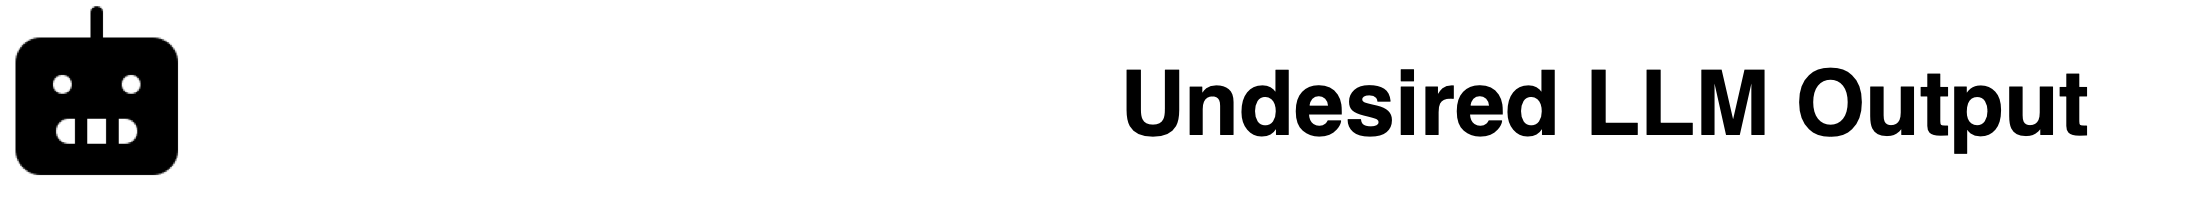
\includegraphics[height=0.8cm]{Images/robot-distance.png} \\
\cellcolor{mistyrose} <VAR>example.output</VAR> \\ 
\end{tabular}
};
\draw [rounded corners=.5em] (table2.north west) rectangle (table2.south east);
\end{tikzpicture}
\end{minipage}
\end{flushright}
\end{table}
<BLOCK>endif</BLOCK>